%By Liping Wang at 2019-09-21
%Contact wangliping2019@ia.ac.cn
\documentclass{article}
\usepackage[UTF8]{ctex}
\usepackage{amsmath}
\usepackage{hyperref}
\usepackage{fancyhdr}
\usepackage{bbm}
\usepackage{graphicx}
\usepackage{url}

\topmargin=-0.45in
\evensidemargin=0in
\oddsidemargin=0in
\textwidth=6.5in
\textheight=9.0in
\headsep=0.25in
\linespread{1.1}



%配置区
\newcommand{\courseName}{算法设计与分析}
\newcommand{\homeworkId}{\#3} %作业编号
\newcommand{\homeworkTitle}{作业\homeworkId}
\newcommand{\studentId}{201928015059003}%学号
\newcommand{\studentName}{杨天健}%姓名


\newcommand{\question}[1]{\section*{Question #1}}
\renewcommand{\part}[1]{\subsection*{(#1)}}



\pagestyle{fancy}
\lhead{\studentName}
\rhead{\courseName\homeworkTitle}
\cfoot{\thepage}

\title{
    \vspace{2in}
    \textmd{\textbf{\courseName}:\homeworkTitle}\\
    \vspace{0.1in}
    \large{\studentId}\\
    \large{\studentName}\\
    \vspace{3in}
}

\begin{document}

\pagenumbering{gobble}
\maketitle
\date{}
\pagebreak


\question{1}
I've uploaded all of my code to \url{https://github.com/yangtianjian/Typical_algorithms}. The core code is in simple\_algorithm/Sorting.hpp. In main function, main.cpp, you can uncomment the two lines: test\_mergesort and test\_quicksort. Don't forget to modity the parameter 'PATH' to fit for your local environment.

\question{2}
I've made a comparison between linked merge sort and quicksort. For each algorithm, there are two cases. For one case, data are provided in random permutation. For another, it is given reversely. The result is provided below and \textbf{the time is given in milliseconds}: \par
\begin{align*}
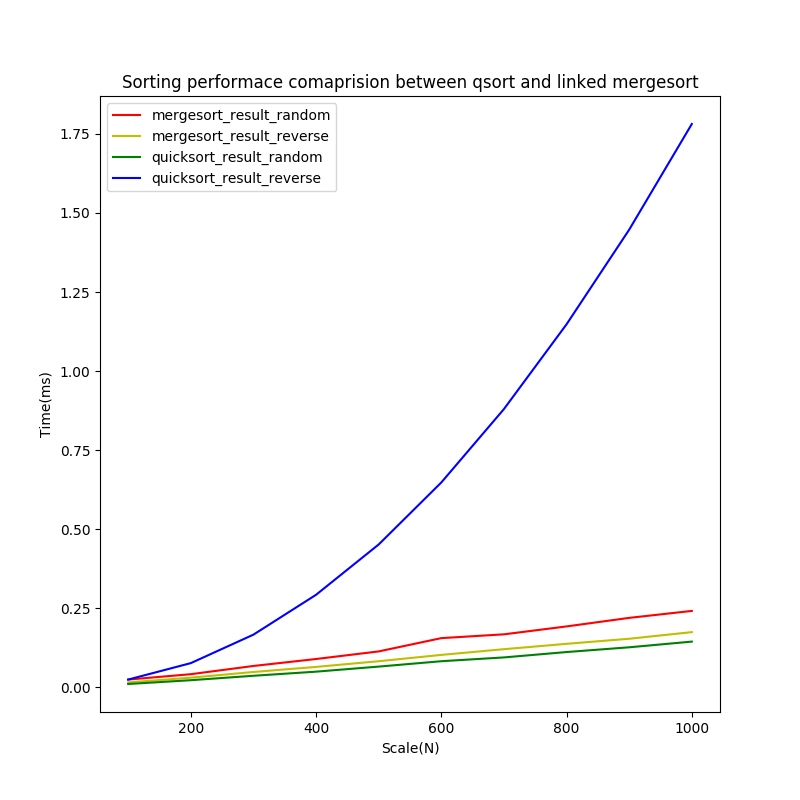
\includegraphics[scale=0.7]{sorting_comparison.png}
\end{align*}

\question{3}
Whether we use an auxiliary array or a linked list, merge sort cannot be finished in-place. Another $n$-size of space is needed. Let's use $f(n)$ to indicate global variables, $g(n)$ for local variables and $T(n)$ for total space complexity. We have:
\begin{align*}
  f(n) &= 2n = \Theta(n) \\
  g(n) &= 2g(\frac{n}{2}) + \Theta(1) \, \Rightarrow \, g(n) = \Theta(n)
\end{align*} \par
So $T(n) &= f(n) + g(n) = \Theta(n)$. \\

\question{4}
Now we use induction method to prove the formula in the question that:
\begin{align}
  R[n] \leq 4cn
\end{align} \par
The precondition is (Here we get rid of serveral unnecessary notations to make it more clearly),
\begin{align}
  C[n][k] &\leq cn + \frac{1}{n} \bigg( \displaystyle\sum_{1 \leq i < k} C[n - i][k - i] + \displaystyle\sum_{k < i \leq n} C[i - 1][k] \bigg) \\
  R[n] &= max_k (C[n][k]) \\
  c &\geq R[1]
\end{align} \par
To begin with, for $n = 1$, $R[1] \leq c \leq 4c$, it is true for (1). \par
Now we have $R[p] \leq 4cp$ for each $p = 1, 2, 3, ..., n - 1$. And we start to prove. \par
Because $R[n] &= max_k (C[n][k])$, for every $k$, $C[n][k] \leq R[n]$. So (2) can be written as:
\begin{align}
  C[n][k] &\leq cn + \frac{1}{n} \bigg( \displaystyle\sum_{1 \leq i < k} C[n - i][k - i] + \displaystyle\sum_{k < i \leq n} C[i - 1][k] \bigg) \\
  &\leq cn + \frac{1}{n} \bigg( \displaystyle\sum_{1 \leq i < k}R[n - i] + \displaystyle\sum_{k < i \leq n} R[i - 1] \bigg)
\end{align} \par
For each $1 \leq i < k$, $n - i \leq n - 1$. And for each $k < i \leq n$, $i - 1 \leq n - 1$. By using former iteration of induction, we have $R[n - i] \leq 4c(n - i)$ and $R[i - 1] \leq 4c(i - 1)$. From(6), we come to:
\begin{align}
  & cn + \frac{1}{n} \bigg( \displaystyle\sum_{1 \leq i < k}R[n - i] + \displaystyle\sum_{k < i \leq n} R[i - 1] \bigg) \\
  &\leq cn + \frac{1}{n} \bigg( \displaystyle\sum_{1 \leq i < k}4c(n - i) + \displaystyle\sum_{k < i \leq n} 4c(i - 1) \bigg) \\
  &= cn + \frac{2c}{n} \bigg[ (2n - k)(k - 1) + (k + n - 1)(n - k) \bigg]
\end{align} \par
In the bracket is a quadratic polynomial respect to k. When $\frac{n + 1}{2}$, the formula can be written as:
\begin{align}
  &cn + \frac{2c}{n} \bigg[ (2n - k)(k - 1) + (k + n - 1)(n - k) \bigg] \\
  & \leq cn + \frac{2c}{n} \bigg[ \frac{1}{2}(n + 1)^2 + n^2 \bigg] - 6c \\
  & \leq cn + \frac{2c}{n} \frac{2}{3} - 6c \\
  &= 4cn + (\frac{2}{n} - 4)c \\
  & \leq 4cn
\end{align} \par
$C[n][k] &\leq 4cn$ for each $k = 1, 2, ..., p - 1$, So we have $R[n] &= max_k (C[n][k]) \leq 4cn$. So the problem is solved.

\end{document}
